% Asset ID: AS2ForcesTikZ-011
% Source: Chapter 5/7 Forces Transcript
% Related lesson section: Worked Example 5
% Purpose: Show how tan alpha = 3/4 gives sine and cosine.
\documentclass[tikz,border=8pt]{standalone}
\usepackage{amsmath}
\usetikzlibrary{arrows.meta, angles, quotes, decorations.pathmorphing}
\begin{document}
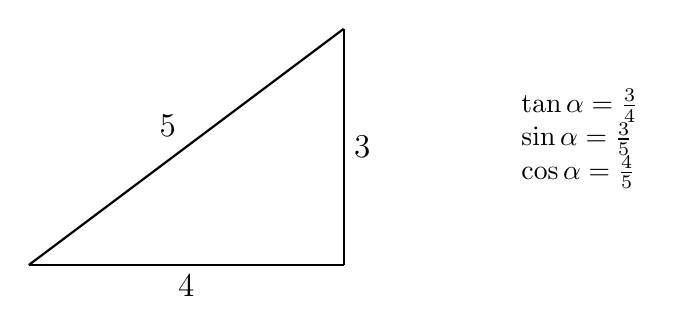
\begin{tikzpicture}[force/.style={-{Latex[length=3mm]}, thick}, comp/.style={-{Latex[length=3mm]}, thick, dashed}, label/.style={font=\large}, note/.style={font=\normalsize}]

\coordinate (A) at (0,0); \coordinate (B) at (4,0); \coordinate (C) at (4,3); \draw[thick] (A)--(B) node[midway,below,label] {$4$}; \draw[thick] (B)--(C) node[midway,right,label] {$3$}; \draw[thick] (A)--(C) node[midway,above left,label] {$5$}; \node[note,align=left] at (7,1.6) {$\tan\alpha=\frac34$\\$\sin\alpha=\frac35$\\$\cos\alpha=\frac45$};
\end{tikzpicture}
\end{document}
